% % no answer key
% \documentclass[letterpaper]{exam}

% answer key
\documentclass[letterpaper, landscape]{exam}
\usepackage{2in1, lscape} 
\printanswers{}

\usepackage{units} 
\usepackage{xfrac} 
\usepackage[fleqn]{amsmath}
\usepackage{cancel}
\usepackage{float}
\usepackage{mdwlist}
\usepackage{booktabs}
\usepackage{cancel}
\usepackage{polynom}
\usepackage{caption}
\usepackage{fullpage}
\usepackage{comment}
\usepackage{enumerate}
\usepackage{graphicx}
\usepackage{parskip}

\everymath{\displaystyle}


\title{Statistics \\ Homework Six}
\date{\today}
\author{}

\begin{document}

  \maketitle

  \section{Homework}
    \begin{itemize*}
      \item read Chapter 6 
      \item exercises: 19--24, 27, 29--31
    \end{itemize*}

  \ifprintanswers{}
    \begin{description}

      \item[19] Table~\ref{tab:ex19} shows the success rate for each treatment. 
        Figure~\ref{fig:ex19} shows the same thing in a bar graph.

        \begin{figure}[H]
          \centering
          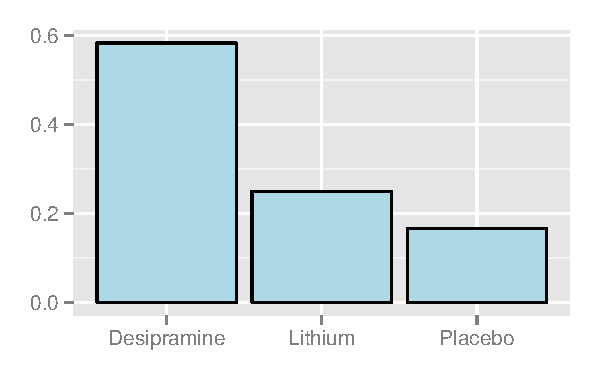
\includegraphics[scale = 0.7]{figures/ex19.pdf}
          \caption{Exercise 19}\label{fig:ex19}
        \end{figure}

        \begin{table}[H]
          \centering
          \begin{tabular}{lr}
            \toprule
            Treatment   & Success Rate \\
            \midrule
            Lithium     & 25\% \\
            Placebo     & 17\% \\
            Desipramine & 58\% \\
            \bottomrule
          \end{tabular}
          \caption{Exercise 19}\label{tab:ex19}
        \end{table}

      \item[20] 
        Table~\ref{tab:ex20a} shows the percentage of men in each job grade.
        Table~\ref{tab:ex20b} shows the percentage of men in each marital status.
        
        \begin{table}[H]
          \centering
          \begin{tabular}{lr}
            \toprule
            Job Grade & Percent \\
            \midrule
            grade 1   & 12\% \\
            grade 2   & 51\% \\
            grade 3   & 30\% \\
            grade 4   & 7\% \\
            \bottomrule
          \end{tabular}
          \caption{Percent of men in each job grade.}\label{tab:ex20a}
        \end{table}

        \begin{table}[H]
          \centering
          \begin{tabular}{lr}
            \toprule
            Marital Status & Percent \\
            \midrule
            single         & 4\% \\
            married        & 94\% \\
            divorced       & 2\% \\
            widowed        & 1\% \\
            \bottomrule
          \end{tabular}
          \caption{Percent of men in each marital status.}\label{tab:ex20b}
        \end{table}
      The percentages might not add up to exactly 100\% because of rounding, but
      they should be close.
      
    \newpage

    \item[21]
      There are 58 single men with grade 1 jobs and 955 grade 1 jobs, 
      \[
        58/955 \approx 6 \%
      \]
      of the grade 1 jobs are held by single men.

      There are 58 single men with grade 1 jobs and 337 single men, 
      \[
        58/337 \approx 17 \% 
      \]
      of the single men hold grade 1 jobs.

    \item[22]
      Table~\ref{tab:ex22} contains the percentage of single men in each job
      grade.

      The percentages should add up to approximately 100\%, although there may
      be some rounding error.

      \begin{table}[H]
        \centering
        \begin{tabular}{lr}
          \toprule
          job grade & percentage \\
          \midrule
          grade 1   & 17\%  \\
          grade 2   & 66\%  \\
          grade 3   & 15\%  \\
          grade 3   & 2\%   \\
          \bottomrule
        \end{tabular}
        \caption{Percentage of single men in each job grade}.\label{tab:ex22}
      \end{table}


    \item[23]
      \begin{enumerate}[(a)]
        \item There are 7730 married men and only 337 single men, so you would expect
        more married men than single men in all the job categories.

        \item 

          \begin{table}[H]
            \centering
            \begin{tabular}{lrrrr}
              \toprule
                       & grade 1 & grade 2 & grade 3 & grade 4 \\
              \midrule
              single   & 17.2\%  & 65.9\%  & 14.8\%  & 2.1\% \\
              married  & 11.3\%  & 50.8\%  & 31.0\%  & 6.9\% \\
              divorced & 11.9\%  & 55.6\%  & 27.0\%  & 5.6\% \\
              widowed  & 19.0\%  & 47.6\%  & 23.8\%  & 9.5\% \\
              \bottomrule
            \end{tabular}
          \end{table}

          There are more single men than married or divorced in grade 1 job.  
          Single men tend to be younger, so this just means the single men tend to
          have the entry-level jobs.  There are few single men with grade 4 jobs,
          which makes sense for the same reason.

          The widowed category doesn't fit the pattern, but there are very few
          widowed men, so there probably isn't a large enough sample size to get a
          good picture of the widowed men.

        \end{enumerate}

    \item[24] As you get older, you tend to make more money.  As you get older, you
      are also more likely to get married.  Age is probably the lurking variable.

    \item[27]
      Table~\ref{tab:ex27} shows the percentage of people in each job for each
      education level.  The more education you have, the more freedom you have
      in organizing your work.

      \begin{table}[H]
        \centering
        \begin{tabular}{lrrr}
          \toprule
                & grade 1 & grade 2 & grade 3     \\
          \midrule
          No HS & 24.4    & 38.6    & 37.0 \\
          HS    & 29.7    & 49.6    & 20.7 \\
          BA    & 45.0    & 47.2    & 7.8  \\
          \bottomrule
        \end{tabular}
        \caption{Percentage of people in each job for each education level.}\label{tab:ex27}
      \end{table}

    \newpage

    \item[29]
      According to Table~\ref{tab:ex29}, women earn A higher percentage of each
      type of degree.  
      
      The gap narrows with the more advanced degrees. Women are a large majority
      of Associate's, Bachelor's, and Master's degrees and only a narrow
      majority of professional and Doctoral degrees.

      \begin{table}[H]
        \centering
        \begin{tabular}{lrr}
          \toprule
                       & F    & M \\
          \midrule
          Associate's  & 63\% & 37\% \\
          Bachelor's   & 59\% & 41\% \\
          Master's     & 61\% & 39\% \\
          Professional & 53\% & 47\% \\
          Doctor's     & 51\% & 49\% \\
          \bottomrule
        \end{tabular}
        \caption{Percentage of each degree earned by men and women}\label{tab:ex29}
      \end{table}

    \item[30]
      % Table \ref{tab:ex30a} shows the cancer levels for each type of patient in
      % the survey.  For example, people with low oil consumption have a 19.7\%
      % rate of color cancer for the participants in the survey.  

      % This table isn't particularly useful, however, because the number of
      % people in each group (colon/control/rectal) is different and this is
      % reflected in the percentages.

      % \begin{table}[H]
      %   \centering
      %   \begin{tabular}{lrrr}
      %     \toprule
      %              & colon  & control & rectal \\
      %     \midrule
      %     low oil  & 19.7\% & 67.9\%  & 12.4\% \\
      %     med oil  & 19.7\% & 68.3\%  & 12.0\% \\
      %     high oil & 20.7\% & 67.9\%  & 11.4\% \\
      %     \bottomrule
      %   \end{tabular}
      %   \caption{Cancer rate for each oil consumption rate}.
      %   \label{tab:ex30a}
      % \end{table}

      Table~\ref{tab:ex30b} shows the oil consumption for each type of patient.
      The oil consumption seems to be very equally divided between the three
      groups.  About a third of the people are in the low/medium/high
      categories, regardless of whether they have cancer or not.

      If eating olive oil prevented cancer, you would expect that the percentage
      of people with high oil consumption and cancer would be lower than the
      percentage of people with high oil consumption and no cancer.

      \begin{table}[H]
        \centering
        \begin{tabular}{lrrr}
          \toprule
                  & high oil & low oil & med oil \\
          \midrule
          colon   & 35.1\%   & 32.5\%  & 32.4\% \\
          rectal  & 32.6\%   & 34.3\%  & 33.1\% \\
          control & 33.9\%   & 32.9\%  & 33.1\% \\
          \bottomrule
        \end{tabular}
        \caption{Oil consumption for each category of patient}.\label{tab:ex30b}
      \end{table}


    \item[31]
      Table~\ref{tab:ex31} shows the heart disease rate for each anger category.
      The more angry you are, the more likely it is that you'll get hear
      disease.

      \begin{table}[H]
        \centering
        \begin{tabular}{rlrr}
          \toprule
                         & No CHD   & CHD \\
          \midrule
          low anger      & 98.3\%   & 1.7\% \\
          moderate anger & 97.7\%   & 2.3\% \\
          high anger     & 95.7\%   & 4.3\% \\
          \bottomrule
        \end{tabular}
        \caption{Heart disease rates for each anger rate.}\label{tab:ex31}
      \end{table}

  \end{description}

  \else
    \vspace{10 cm}
    \begin{quote}
      \begin{em}
        I would encourage people to look around them in their community and find an
        organization that is doing something that they believe in, even if that
        organization has only five people, or ten people, or twenty people, or a hundred
        people. And to look at history and understand that when change takes place it
        takes place as a result of large, large numbers of people doing little things
        unbeknownst to one another
      \end{em}
    \end{quote}
    \hspace{1 cm} --Howard Zinn
  \fi

\end{document}

